\chapter{DAGs}
\label{chapt:DAGs}
Let's introduce the DAGs or Directed Acyclic Graph, we will need this powerful tool to model causal relationships that wont be properly defined until chapter \ref{chapt:PotentialOM}.
A DAG is a graph that represents the set of random variables $ V = (V_1,..., V_m)$ as nodes and the casual connection between them as edges. It's called "Directed" because the graph can't form loops so it's not suited to describe simultaneous reciprocal causal relationships or feedback loop, such as: $A \leftrightarrow B $, even if some extension of the model allow this kind of interaction, it is advised not to use this kinds of graphs \citep{cunningham2021causal}.

show examples of valid and invalid dags



%
%\begin{figure}[ht]
%  \subcaptionbox{Non valid DAG}[.22\linewidth]{%
%	\begin{tikzpicture}
%		\node (A) at (0,0) {$A$};
%    		\node (B) at (1,0) {$B$};
%    		\path[<-] (A) edge (B);
%    		\path[->] (B) edge (A);
%	\end{tikzpicture}
%  }%
%  \subcaptionbox{Non valid DAG}[.22\linewidth]{%
%	\begin{tikzpicture}
%		\node (A) at (0,0) {$A$};
%    		\node (B) at (1,0) {$B$};
%    		\path[<-] (A) edge (A);
%    		\path[->] (B) edge (A);
%	\end{tikzpicture}
%  }
%  \subcaptionbox{Valid DAG}[.22\linewidth]{%
%	\begin{tikzpicture}
%		\node (A) at (0,0) {$A$};
%    		\node (B) at (1,0) {$B$};
%    		\node (C) at (2,0) {$C$};
%    		\path[<-] (A) edge (B);
%    		\path[->] (B) edge (C);
%    		
%	\end{tikzpicture}
%  }%
%	\label{validDAG}
%
%\end{figure}
%(I grafi sono da rifare)
%
%Bisogna inoltre dire che i DAGs, essendo dei grafi sono di natura più sintetici, contengono molte informazioni non solo grazie agli archi disegnati ma anche grazie a quelli \textbf{non} disegnati, ad esempio il DAG \ref{validDAG} implica che $A \perp\!\!\!\perp C$ visto che non esiste un arco che li colleghi. 
%
% %Bisogna essere molto vigili delle assunzione nascoste di un DAG.



\section{Nodes and Edges}
In this section we will show examples of a DAGs where C is the variable of interest or \textit{outcome} variable for a statistical analysis (years lived after surgery). A is the exposure variable or the variable for which we want to identify the causal effect on the \textit{outcome} variable. We do this to introduce terminology necessary to describe properties of this model.
\subsection{Nodes}

\subsubsection{Descendants Ancestors Parents and Child}
We call parents (denoted as $PA_m$) the set of causal variables that have a directed arrow in to $V_m$. We call ancestor any variable witch through a sequence of nodes connected by directed edges. The opposite definition goes for kids and ancestors. 

\begin{figure}[H]
\centering    
	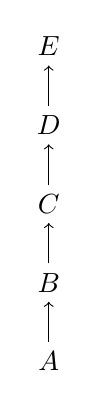
\begin{tikzpicture}
		\node (A) at (0,0) {$A$};
    		\node (B) at (0,1) {$B$};
    		\node (C) at (0,2) {$C$};
    		\node (D) at (0,3) {$D$};
    		\node (E) at (0,4) {$E$};
		\path[->] (A) edge (B);
    		\path[->] (B) edge (C);
    		\path[->] (C) edge (D);s
    		\path[->] (D) edge (E);
	\end{tikzpicture}
\caption{DAG: Common effect}
\label{DAG:term}
\end{figure}

In the DAG \ref{DAG:term} for C : 
\begin{itemize}
\item {A, B} are it's ancestors
\item {B} is it's parent
\item {D, E} are it's descendants
\item {D} is it's child
\end{itemize}
Note that {A, B} are only C's ancestors not is descendants because the directed arrow goes from {A , B} to C. 
We can say from this graph that A caused B that caused C and so on, so by the graph we understand that the treatment had an effect on the health of at least one individual that was \textit{mediated} through B.

\subsubsection{Mediators , Common effects , Common causes }
Let's focus on B and all the possible connection between B and A and C:
\begin{figure}[H]
\centering    
	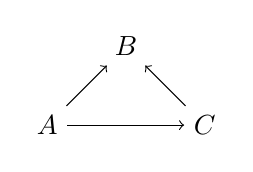
\begin{tikzpicture}
		\node (A) at (0,0) {$A$};
    		\node (B) at (1,1) {$B$};
    		\node (C) at (2,0) {$C$};
		\path[->] (A) edge (B);
    		\path[<-] (B) edge (C);
    		\path[->] (A) edge (C);
	\end{tikzpicture}
\caption{DAG: Common effect}
\label{DAG:Common effect}
\end{figure} 
\begin{figure}[H]
	\centering
	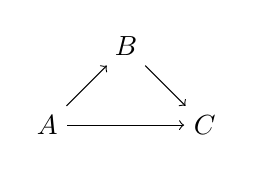
\begin{tikzpicture}
		\node (A) at (0,0) {$A$};
    		\node (B) at (1,1) {$B$};
    		\node (C) at (2,0) {$C$};
    		\path[->] (A) edge (B);
    		\path[->] (B) edge (C);
		\path[->] (A) edge (C);
	\end{tikzpicture}
\caption{DAG: Mediator}
\label{DAG:Mediator}
\end{figure} 
\begin{figure}[H]
	\centering
	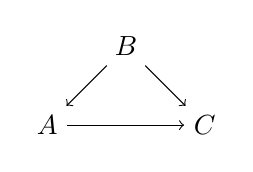
\begin{tikzpicture}
		\node (A) at (0,0) {$A$};
    		\node (B) at (1,1) {$B$};
    		\node (C) at (2,0) {$C$};
    		\path[<-] (A) edge (B);
    		\path[->] (B) edge (C);
    		\path[->] (A) edge (C);
	\end{tikzpicture}
\caption{DAG: Common cause}
\label{DAG:Common cause}
\end{figure}
In the graph \ref{DAG:Common effect} B is a common effect of the surgery and the health of the patient, these kind of nodes are called \textit{colliders}.  It has to be noted though that in the graph we don't have any information about the nature of the interaction of the two causes or the strength of the causal relationship.
In the graph \ref{DAG:Mediator} B is the mediator, for witch the causal effect passes through, in this example let B be the presence of tumour and let's say that all operation A remove successfully the tumour the causal effect of the operation is mediated by the presence of the tumor itself. As a general rule if the mediator's descendants don't have has a common cause the \textit{exposure} and the \textit{outcome}, mediators can be ignored, the reason for this will be fully explained later.
Meanwhile in the graph \ref{DAG:Common effect} B is the common cause of both the \textit{exposure} and the \textit{outcome}, for example B could be inflammation and this both caused people to opt in for the surgery and is the cause of a faster death, we can see that this kind of relationship is the most problematic because any association between better health is \textit{spurious}, this kinds of nodes are called \textit{confounders}.

%
%Infatti se volessimo quantificare la relazione causale tra A e C quando B è un \textit{non collider} o  un \textit{confounder} risulta più difficoltoso perchè sappiamo che B introduce  sistematicamente correlazioni spurie tra A e C (bisogna capire meglio come affrontare i mediators [bisogna controllarli?], osservazione più giusta per i ). Invece nel caso mostrato in figura \ref{DAG:Common effect} potremmo interpretare il $\hat{\delta}$ della regressione lineare:
%\begin{equation}
%C_i= A_i\delta + \epsilon_i
%\end{equation}
%come quantificazione dell'effetto causale che A ha su C, questo lo possiamo affermare solo dopo aver confermato che effettivamente:
%\begin{itemize}
%\item il grafo soddisfa \textit{Backdoor criterion} ( paragrafo \ref{sect:backdoor})
%\item La direzione della causalità è corretta
%\end{itemize}
\subsection{Edges}
To make any further progress with causal inference it is necessary to outline some assumption  \citep{hernan2020causal}: 
\begin{ass}[Markov assumption]
We define the distribution of V to be Markov with respect to a DAG G (equivalently, the distribution factors according to a DAG G) if, for each j, $V_j$ is independent of its non-descendants conditional on its parent.
\end{ass}
This may seem an innocuous assumption but it is a very strong one, because it means that for two variable $V_j$ $V_m$ if there isn't a directed edge between the two then $V_j \perp\!\!\!\perp V_m | (PA_j, PA_m)$.
We can show this as $V_j \perp\!\!\!\perp _G V_m | (PA_j, PA_m) \rightarrow V_j \perp\!\!\!\perp _G V_m | (PA_j, PA_m)$.

 It's the analyst burden to assert on a case to case basis that this condition  is indeed credible.
Another 


definizione di open backdoor 

elenco di tutte le path possibili  con esempio




% magari metterli di fianco
%\begin{figure}[ht]
%  \subcaptionbox{First subfigure}[.22\linewidth]{%
%	\begin{tikzpicture}
%		\node (A) at (0,0) {$A$};
%    		\node (B) at (1,0) {$B$};
%    		\node (C) at (2,0) {$C$};
%    		\path[<-] (A) edge (B);
%    		\path[->] (B) edge (C);
%	\end{tikzpicture}
%  }%
%  \hfill
%  \subcaptionbox{Second subfigure}[.22\linewidth]{%
%	\begin{tikzpicture}
%		\node (A) at (0,0) {$A$};
%    		\node (B) at (1,0) {$B$};
%    		\node (C) at (2,0) {$C$};
%    		\path[<-] (A) edge (B);
%    		\path[->] (B) edge (C);
%	\end{tikzpicture}
%  }
%  \subcaptionbox{First subfigure}[.22\linewidth]{%
%	\begin{tikzpicture}
%		\node (A) at (0,0) {$A$};
%    		\node (B) at (1,0) {$B$};
%    		\node (C) at (2,0) {$C$};
%    		\path[<-] (A) edge (B);
%    		\path[->] (B) edge (C);
%	\end{tikzpicture}
%  }%
%
%\end{figure}

\section{Back door criterion}
\label{sect:backdoor}


\section{Collider Bias}
\begin{figure}[H]
\centering
	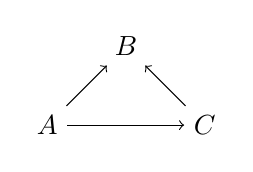
\begin{tikzpicture}
		\node (A) at (0,0) {$A$};
    		\node (B) at (1,1) {$B$};
    		\node (C) at (2,0) {$C$};
		\path[->] (A) edge (B);
    		\path[<-] (B) edge (C);
    		\path[->] (A) edge (C);
	\end{tikzpicture}
\caption{DAG:collider bias}
\label{DAG:Colliderbias}
\end{figure} 



Markov assumption
